%%%%%%%%%%%%%%%%%%%% Chapter 2
%\chapter{Related works} % Main chapter title
%\label{Chapter2} % For referencing the chapter elsewhere, use 
%----------------------------------------------------------------------------------------
\section*{Chapter summary}
\noindent
This chapter reviews developments in adaptive and enveloping grasping, with emphasis on loop- and belt-based grippers, sensorized soft grippers, material and microstructure innovations, and grasp planning algorithms. The survey synthesizes how these approaches trade off shape adaptability, load capacity, and sensing complexity.

\noindent
The literature suggests that loop-based grippers offer strong advantages in distributed contact and tolerance to positional uncertainty, but they require robust sensing and routing strategies to handle dynamic targets and scale to diverse applications — issues the Lasso Gripper prototype seeks to explore.

\section{Development of Adaptive Grasping and its application}
\subsection{The Necessity of Enveloping and Encircling Grasping}
Enveloping and encircling grasping provide enhanced stability and shape adaptability for a wide range of objects. This subsection reviews recent structural and control approaches that achieve enveloping grasps and highlights the remaining limitations that motivate loop-based and tendon-driven solutions.

One notable study introduces a dual-mode soft robotic gripper designed with integrated  annular structures and a contraction actuator. This design significantly improves shape tolerance and gripping force by altering the contact method between the gripper and the object, adjusting the stiffness and load capacity through controlled material properties \cite{hu2023dual}.

Another novel technique employs a soft gripper that leverages a belt loop with an actuated adhesion mechanism. This mechanism provides dual-directional force – both radial and tangential – which enhances the effectiveness and stability of the grasping action. The minimal interaction force strategy ensures gentle handling, making it suitable for fragile objects \cite{chen2024soft}.

Additional studies introduce an affordable, underactuated compliant gripper capable of adapting to objects of diverse sizes and shapes. The design features a flexure motion transmission mechanism and multifunctional jaws, allowing for a more conforming grasp. This interaction between the gripper and the target object increases both gripping force and stability \cite{sun2024low}.

Additionally, a study on a tendon-driven robotic gripper highlights the importance of stable enveloping grasps. By optimizing tendon routes and stiffness, this gripper can perform multiple grasping modes, including parallel, enveloping, and fingertip grasps. This versatility ensures the gripper's flexibility and stability across various applications \cite{ciocarlie2014velo}.

Enveloping and encircling grasping techniques are crucial in robotic grasping technology. They enhance shape adaptability, gripping force, and stability, providing robust support for robots in complex and dynamic environments.
\begin{figure}[htbp]
\centering
\begin{tabular}{cc}
\begin{minipage}[t]{0.5\textwidth}
\centering
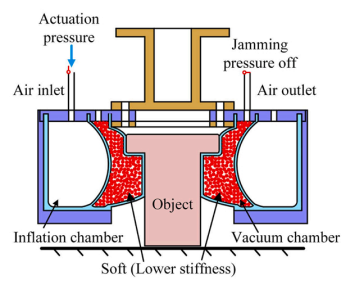
\includegraphics[width=0.7\columnwidth]{Figures/1.png}
\caption{Pressurized the actuation chamber and adaptive grasping \cite{hu2023dual}}
\end{minipage}
\qquad
\begin{minipage}[t]{0.5\textwidth}
\centering
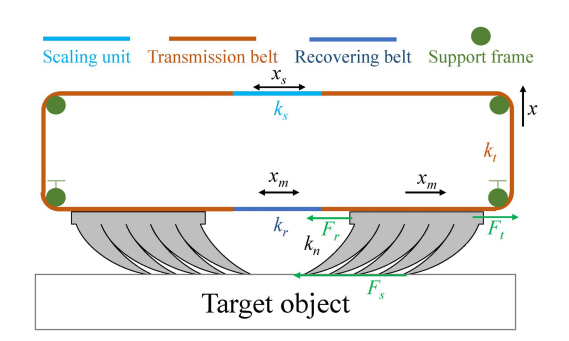
\includegraphics[width=0.7\columnwidth]{Figures/8.png}
\caption{Belt Loop Actuated Adhesion Design \cite{chen2024soft}}
\end{minipage}
\end{tabular}
\begin{tabular}{cc}
\begin{minipage}[t]{0.5\textwidth}
\centering
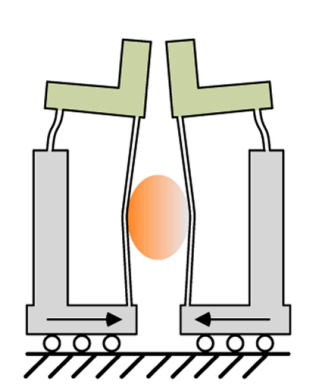
\includegraphics[width=0.7\columnwidth]{Figures/4.png}
\caption{Enveloping grasps of the multifunctional jaw \cite{sun2024low}}
\end{minipage}
\qquad
\begin{minipage}[t]{0.5\textwidth}
\centering
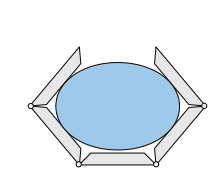
\includegraphics[width=0.7\columnwidth]{Figures/172.png}
\caption{Examples of enveloping grasps of Velo gripper \cite{ciocarlie2014velo}}
\end{minipage}
\end{tabular}
\end{figure}





\subsection{Grasping System with Integrated Sensors}

The integration of sensors with soft materials such as loops significantly enhances the efficiency and adaptability of robotic grasping systems. Various studies have demonstrated the potential benefits of combining these elements to improve performance in different contexts.

A notable example is a modular flying gripper that utilizes a loop gripper mechanism to control its position and pose flexibly. This system, composed of quadrotor-based modules, showcases the versatility of encircling grasping techniques. The decentralized control approach enables the flying gripper to modify its aperture angle, thereby facilitating efficient object grasping and transportation \cite{gabrich2018flying}.

In another study, a soft robotic gripper equipped with a liquid-metal sensing skin provides a robust feedback mechanism. This gripper, integrated with proximity, pressure, and orientation sensors, operates using shape-memory alloy springs to transition between open and close states. The closed-loop control enabled by these sensors allows the system to detect and respond to external disturbances, enhancing its grasping, release, and transportation capabilities \cite{yin2020closing}.

Further advancements are seen in the development of a continuum body gripper that incorporates flexible latex bladder sensors. By measuring air pressure changes, these sensors provide tactile and proprioceptive feedback, essential for delicate and high-force grasping. This integration allows the gripper to manage a diverse array of objects, ranging from heavy to fragile items, with minimal control input. The sensorized gripper demonstrates high sensitivity and repeatability, making it a cost-effective and durable solution for universal grasping applications \cite{hughes2020sensorization}.

Additionally, a visual-tactile fusion framework has been proposed to address the challenges of grasping transparent objects in complex environments. This framework combines visual and tactile data to enhance grasping efficiency. A tactile calibration technique combined with a visual-tactile fusion classification method greatly enhances the success rate and accuracy of grasping transparent objects. The experimental results validate the effectiveness of integrating tactile sensors within the gripper system, particularly for objects that are irregular or visually undetectable \cite{li2023visual}.

The combination of sensors with soft materials such as loops in robotic grippers offers significant improvements in grasping systems. These integrations provide enhanced feedback, adaptability, and control, rendering them invaluable for a wide array of applications, from delicate object handling to complex environmental interactions.

\begin{figure}[htbp]
\centering
\begin{tabular}{cc}
\begin{minipage}[t]{0.5\textwidth}
\centering
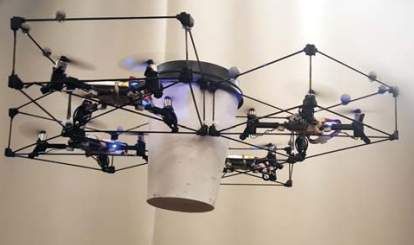
\includegraphics[width=0.7\columnwidth]{Figures/2.png}
\caption{The Flying Gripper holding a coffee cup \cite{gabrich2018flying}}
\end{minipage}
\qquad
\begin{minipage}[t]{0.5\textwidth}
\centering
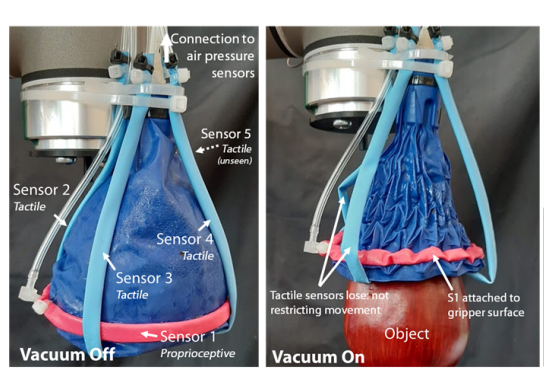
\includegraphics[width=0.7\columnwidth]{Figures/15.png}
\caption{The illustration of tactile sensor and pressure sensors integrated in the loop gripper \cite{hughes2020sensorization}}
\end{minipage}
\end{tabular}
\end{figure}



\subsection{Designing for the Physical Properties of Soft Gripper}

Through advancements in material technology and microstructural design, significant progress has been made in altering the physical properties of flexible materials like ropes. These innovations have paved the way for the development of more efficient and adaptable soft robotic grippers.

A groundbreaking soft gripper utilizing a self-sensing super-coiled polymer (SCP) actuator is introduced by Wang et al. (2021). This actuator is crafted from multi-strand sewing thread that undergoes a self-coiling process, enabling it to untwist when heated. The addition of a metal wire wrapped around the SCP enhances temperature measurement precision, forming a closed-loop control system for accurate gripper manipulation. This approach offers a foundation for customizing the physical properties of rope-like materials for actuator applications \cite{wang2021lightweight}.

Sun et al. (2020) described a soft gripper with adjustable stiffness, inspired by the behavior of pangolin scales. The gripper is composed of two layers: a variable stiffness layer and a pneumatic-driven layer. The variable stiffness layer emulates pangolin scales, remaining flexible during normal activities but becoming rigid when threatened. The toothed pneumatic actuator increases the gripper's stiffness, enabling it to grasp a wide range of objects effectively. The autonomous control system of this gripper collects feedback signals to adjust the stiffness autonomously, making it suitable for unstructured environments \cite{sun2020soft}.

Zhang et al. (2017) tackled the design problem of soft robots using a topology optimization framework. A pneumatically actuated soft gripper was developed, with three fingers each designed as a continuum compliant mechanism to achieve maximum bending deformation. This actuator was fabricated through 3D printing, and experimental results demonstrated its ability to grasp objects effectively. This optimization approach provides valuable insights for further exploration of the microstructure of lasso grippers \cite{zhang2017design}.

Li et al. proposed a soft gripper inspired by the inchworm's true leg. This design includes two rows of sharp hooks on a soft palm, with connections made via Shape Memory Alloy (SMA) springs. The design allows the gripper to adhere to rough surfaces and grasp objects with varying shapes and dimensions. The combination of elastic muscle-like structures and sharp hooks enhances the load-carrying capacity of the gripper, demonstrating the potential of microstructural design in soft robotics \cite{li2017development}.

Wang et al. (2017) explored the usage of Shape Memory Alloy (SMA) in soft grippers, addressing the inherent softness and low actuation force of traditional systems. The study described a soft gripper with variable stiffness based on SMA, composed of three fingers, each with two hinges. The hinges can achieve a significant change in stiffness, allowing the gripper to adapt to various shapes and weights. This material modification approach shows promise for effective grasping applications \cite{wang2017shape}.

The integration of advanced material technologies and microstructural designs has significantly enhanced the capabilities of soft robotic grippers. These innovations provide a robust foundation for developing adaptable and efficient grasping systems.

\begin{figure}[htbp]
\centering
\begin{tabular}{cc}
\begin{minipage}[t]{1\textwidth}
\centering
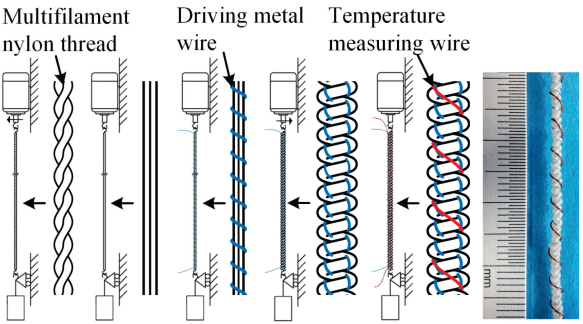
\includegraphics[width=0.7\columnwidth]{Figures/3.png}
\caption{Manufacturing process of actuator with multifilament nylon thread \cite{wang2021lightweight}}
\end{minipage}

\end{tabular}
\begin{tabular}{cc}
\begin{minipage}[t]{0.5\textwidth}
\centering
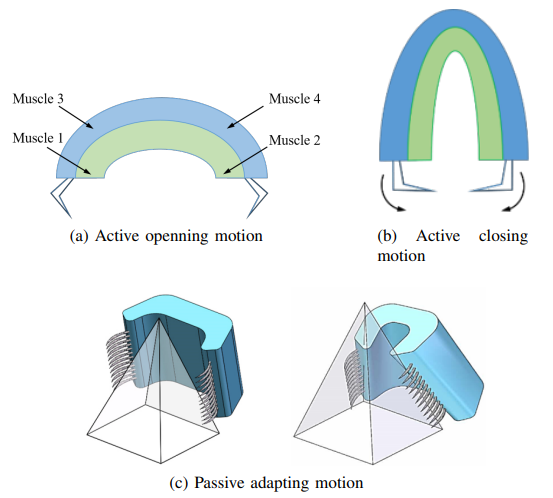
\includegraphics[width=0.7\columnwidth]{Figures/12.png}
\caption{Bio-mechanism of inchworm’s true leg \cite{li2017development}}
\end{minipage}
\qquad
\begin{minipage}[t]{0.5\textwidth}
\centering
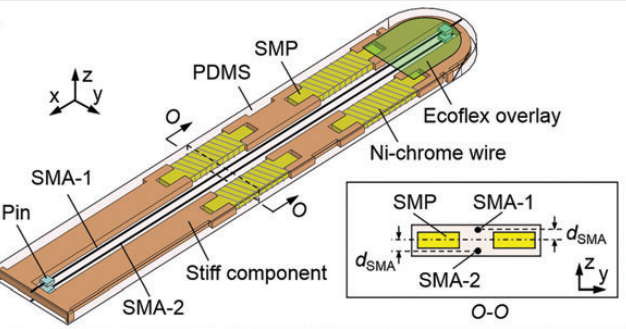
\includegraphics[width=0.7\columnwidth]{Figures/19.png}
\caption{Shape Memory Alloy-Based Soft Gripper \cite{wang2017shape}}
\end{minipage}
\end{tabular}
\end{figure}


\subsection{Advancement of Grasp Planning Algorithm for Lasso Grippers}

The design of grasping algorithms has made significant strides in enhancing the adaptability and efficiency of robotic grippers, particularly those employing rope-like structures such as lasso grippers. These algorithms leverage unique approaches to optimize grasp planning and ensure stable and robust manipulation.

Li et al. (2015) proposed an innovative grasp planning method that addresses the computational challenge of determining stable force-closure grasp configurations for multi-fingered hands. A low-level shape exploration technique is employed in this method by wrapping multiple cords around an object to quickly identify promising grasping regions. Using a variant of the close-until-contact procedure, contact points are determined by the algorithm, which then utilizes finger kinematics and contact information to filter out unstable grasps. This approach not only enhances the natural appearance of grasps but also improves efficiency, as it bypasses extensive preprocessing steps like segmentation and medial axis extraction. The adaptability of this method suggests that the structural concept of wrapping cords around objects can be effectively applied to lasso grippers, potentially offering superior grasping performance \cite{li2015fast}.

Fang et al. (2023) introduced the AnyGrasp algorithm, designed to enhance robust and efficient grasp perception across both spatial and temporal domains. This algorithm utilizes a dense supervision strategy, integrating real perception data with analytic labels to create a comprehensive training dataset. By incorporating object center-of-mass awareness into the learning process, AnyGrasp improves grasp stability. Additionally, it employs grasp correspondence across observations, enabling dynamic tracking of grasp poses, which ensures effectiveness even in noisy environments. The success of AnyGrasp in achieving a high success rate in bin clearing tasks underscores its potential applicability to various robotic grippers, including those with lasso structures \cite{fang2023anygrasp}.

These advancements in grasping algorithm design underscore the importance of innovative computational methods in enhancing the functionality of robotic grippers. The adaptive planning optimization demonstrated by Li et al. (2015) highlights the potential of rope-like structures in improving grasp performance. As the field continues to evolve, integrating these approaches with lasso grippers could lead to more versatile and effective robotic grasping systems.

\begin{figure}[htbp]
\centering
\begin{tabular}{cc}
\begin{minipage}[t]{0.6\textwidth}
\centering
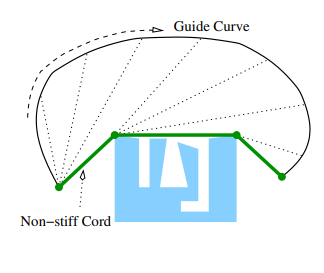
\includegraphics[width=0.7\columnwidth]{Figures/14.png}
\caption{Geometric construction of a non-stiff cord \cite{li2015fast}}
\end{minipage}

\end{tabular}

\end{figure}

\subsection{Application of Lasso Grippers in Real-World Scenarios}

The application of lasso grippers in various real-world scenarios demonstrates their versatility and effectiveness in handling a variety of objects with minimal control effort and high reliability. This section reviews recent advancements and practical implementations of lasso grippers across different fields.

Manes et al. (2024) introduced a soft cable loop-based gripper designed for robotic automation in chemistry laboratories. This gripper can reliably grasp cylindrical and prismatic objects of various sizes with minimal clearance. The design utilizes the compliance of a cable to completely envelop target objects, with support provided by a rigid finger once the grip is secured. This mechanism requires minimal control effort, making it highly practical for repetitive tasks in automated chemistry processes. The gripper demonstrated a grasp reliability with a failure rate of less than 1\%, showcasing its efficacy in handling delicate laboratory glassware. However, the use of a self-supporting plastic polymer material limits the loop size, as larger loops would fail to maintain their shape \cite{manes2024soft}.

\begin{figure}[htbp]
\centering
\begin{tabular}{cc}
\begin{minipage}[t]{1\textwidth}
\centering
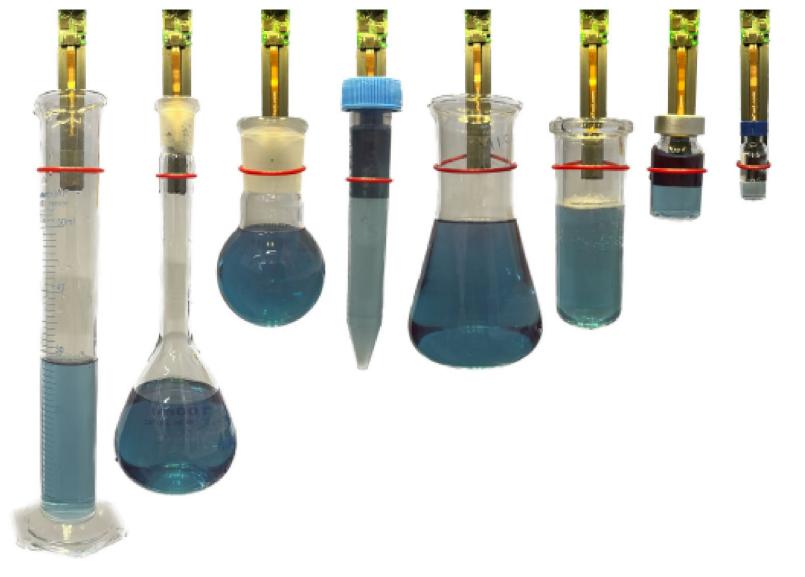
\includegraphics[width=0.7\columnwidth]{Figures/6.png}
\caption{A cable loop gripper prototype was evaluated for its ability to grasp various types of chemistry glassware. \cite{manes2024soft}}
\end{minipage}

\end{tabular}
\begin{tabular}{cc}
\begin{minipage}[t]{0.5\textwidth}
\centering
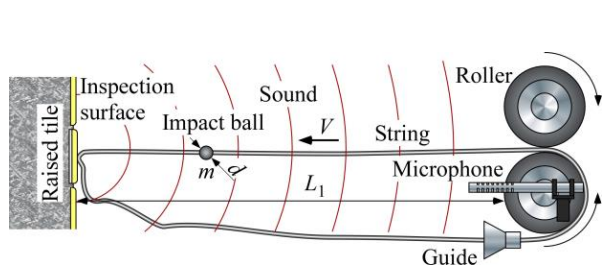
\includegraphics[width=0.7\columnwidth]{Figures/13.png}
\caption{String shoot impact towards a wall \cite{Japan2023}}
\end{minipage}
\qquad
\begin{minipage}[t]{0.5\textwidth}
\centering
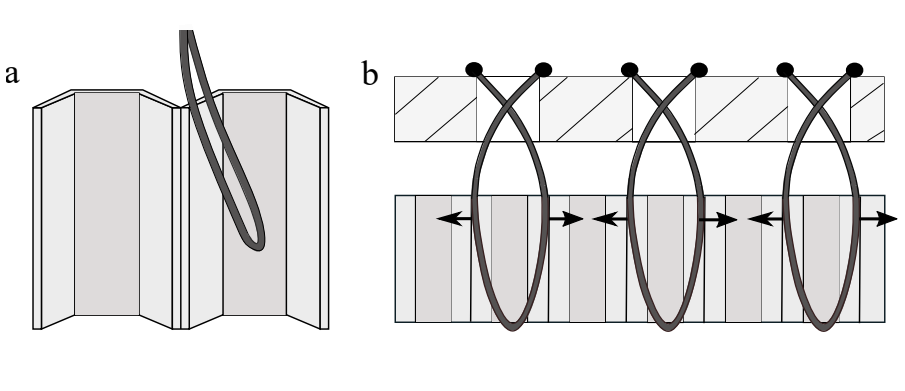
\includegraphics[width=0.7\columnwidth]{Figures/16.png}
\caption{String loop gripper for honeycomb materials \cite{roth2021loop}}
\end{minipage}
\end{tabular}
\end{figure}


A cable-driven gripper with perception capabilities for autonomous strawberry picking was developed by Xiong et al. (2018). The gripper utilizes six fingers to create a closed space around a target strawberry, gently cutting the stem without causing damage to the fruit. Equipped with infrared sensors, positional errors can be corrected by the gripper, enhancing robustness and achieving a high success rate in picking isolated strawberries. The integration of internal perception allows the gripper to tolerate positional inaccuracies, reducing the need for slow, high-level closed-loop control. This design highlights the advantages of using cable actuators, such as flexibility and biological friendliness, making it suitable for delicate agricultural applications \cite{xiong2018design}.

Roth et al. (2021) presented the Loop Gripper designed for handling honeycomb materials used in various industries. This gripper uses adjustable threads to provide the necessary flexibility and sensitivity to grip honeycomb panels without damaging their fragile cell walls. Through a series of tests, the optimal gripping parameters for various honeycomb materials were determined, proving the concept's suitability for automated gripping tasks. The Loop Gripper's approach of using a soft, structure-friendly force to grasp objects aligns with the principles of lasso grippers, emphasizing the importance of adaptability and gentle handling \cite{roth2021loop}.

These studies underscore the practical applications of lasso grippers in diverse fields, from chemistry laboratories to agricultural and material handling tasks. The inherent adaptability and gentle handling capabilities of lasso grippers make them an effective solution for various automated processes, demonstrating their potential for widespread adoption in real-world scenarios.




\subsection{The Balance between Flexibility and Strength}

Current research in robotic gripping mechanisms often focuses on achieving a balance between flexibility and strength. Pneumatic flexible grippers, for instance, offer excellent shape adaptability but are limited in their working range and load capacity. Yu et al. have noted that soft pneumatic actuators are widely utilized in soft robots, where their bending angles and motion rules at different pressures are crucial for practical applications \cite{yu2022modeling}. However, despite their flexibility, these actuators struggle with heavier loads and larger workspaces. Moreover, their dependency on precise pressure control can make them susceptible to performance inconsistencies, particularly in environments where maintaining stable pressure is challenging.

\begin{figure}[htbp]
\centering
\begin{tabular}{cc}
\begin{minipage}[t]{0.9\textwidth}
\centering
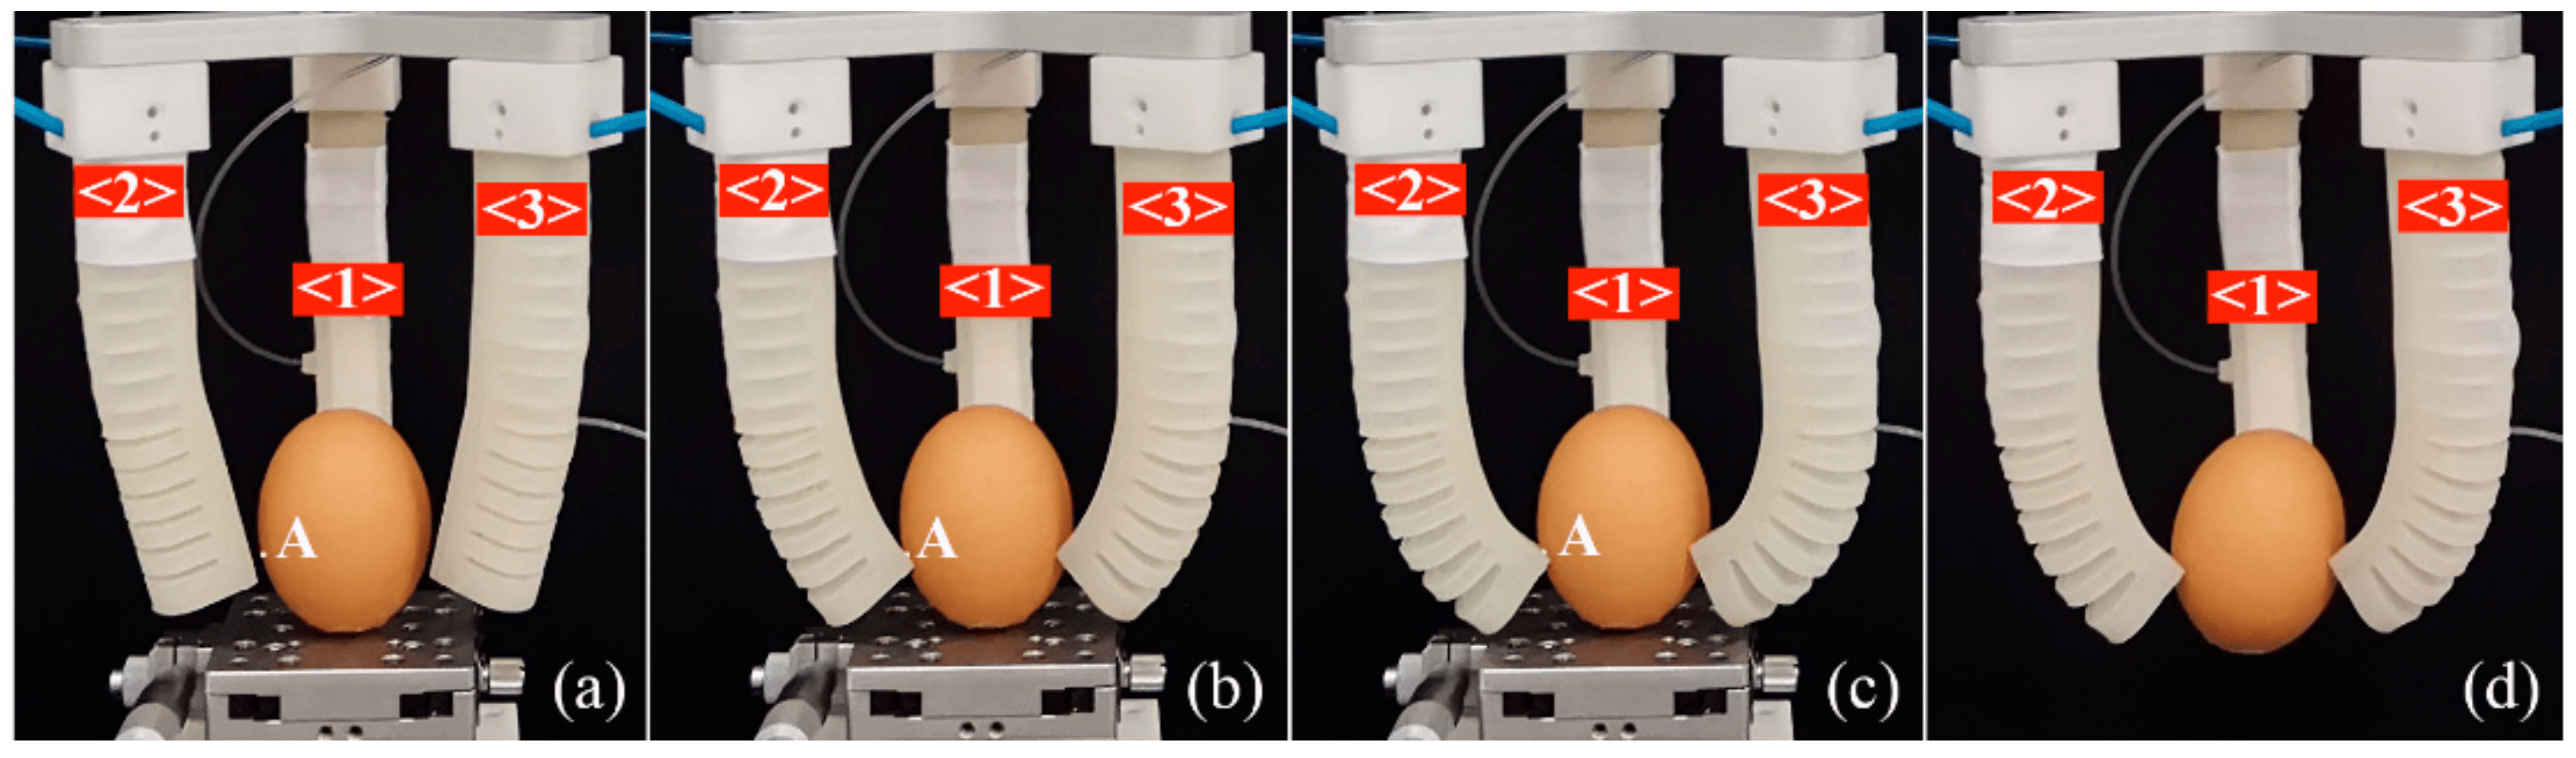
\includegraphics[width=1\columnwidth]{Figures/sensors-22-04851-g014.png}
\caption{Pneumatic actuator grasping process of an egg \cite{yu2022modeling}: (a) The soft actuator moves toward the egg when pneumatic module one is pressurized to 10 kPa, with module two remaining at zero pressure. (b) Contact between the tip of the soft actuator and the egg occurs when the pressure in module one is increased to 20 kPa and module two is set to 14.1 kPa. (c) The egg is securely pinched by the gripper when both module one and module two are pressurized to 20 kPa. (d) The egg is held firmly when the supporting platform is removed, indicating a stable grasp by the gripper.}
\label{linkage structure A}
\end{minipage}
% \qquad
% \begin{minipage}[t]{0.5\textwidth}
% \centering
% \includegraphics[width=0.7\columnwidth]{Figures/linkage structure B.png}
% \caption{Parallel Four-bar Linkage B}
% \label{linkage structure B}
% \end{minipage}
\end{tabular}
\end{figure}

On the other hand, Chameleon-like shooting manipulator offer extended working ranges but suffer from lower success rates and reduced effective working ranges \cite{mochiyama2015chameleon}. Such systems often rely heavily on complex control algorithms and precise timing, which can be difficult to manage in real-time applications, leading to potential delays and reduced effectiveness in fast-paced environments.

\begin{figure}[htbp]
\centering
\begin{tabular}{cc}
\begin{minipage}[t]{0.45\textwidth}
\centering
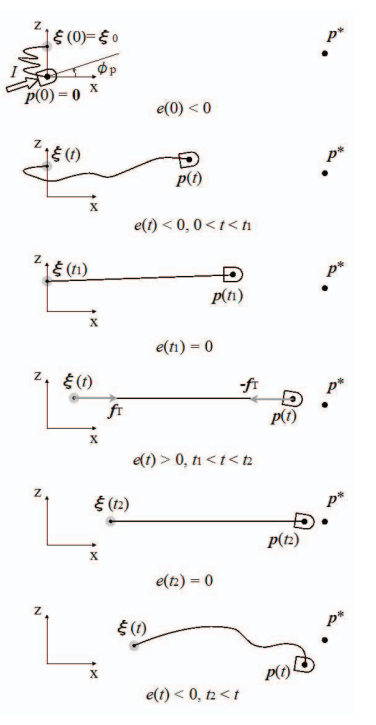
\includegraphics[width=0.8\columnwidth]{Figures/chameleon.png}
\caption{Manipulating model of chameleon-like gripper \cite{mochiyama2015chameleon}.}
\label{linkage structure A}
\end{minipage}
% \qquad
% \begin{minipage}[t]{0.5\textwidth}
% \centering
% \includegraphics[width=0.7\columnwidth]{Figures/linkage structure B.png}
% \caption{Parallel Four-bar Linkage B}
% \label{linkage structure B}
% \end{minipage}
\end{tabular}
\end{figure}

Fractal grippers, as discussed by Tisdale and Burdick, draw inspiration from an older concept called the Fractal Vise \cite{tisdale2023fractal}. Their work emphasizes the gripper's ability to conform passively to various objects using a single actuator. Nonetheless, while these mechanisms offer synergistic properties and adaptability, their integration with existing systems and capacity for high-load tasks are still limited. The passive nature of these grippers, while beneficial in certain contexts, can also lead to a lack of control over the gripping force, making them unsuitable for tasks requiring precise manipulation of heavy or delicate objects.

\begin{figure}[htbp]
\centering
\begin{tabular}{cc}
\begin{minipage}[t]{1.1\textwidth}
\centering
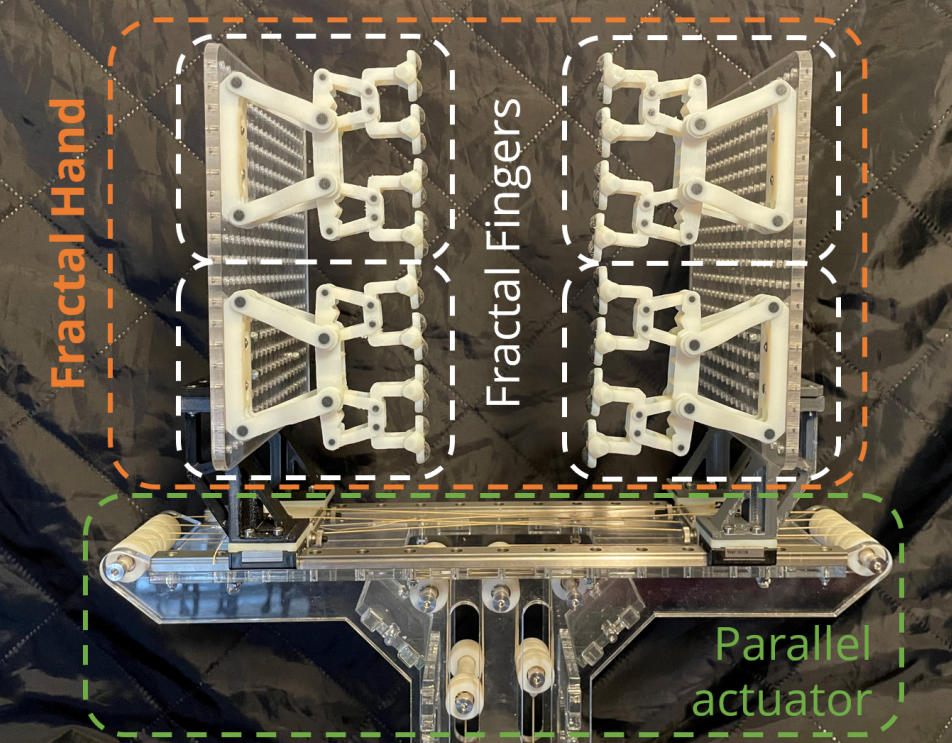
\includegraphics[width=0.8\columnwidth]{Figures/fractal.png}
\caption{ Fractal Hand prototype \cite{tisdale2023fractal}.}
\label{linkage structure A}
\end{minipage}
% \qquad
% \begin{minipage}[t]{0.5\textwidth}
% \centering
% \includegraphics[width=0.7\columnwidth]{Figures/linkage structure B.png}
% \caption{Parallel Four-bar Linkage B}
% \label{linkage structure B}
% \end{minipage}
\end{tabular}
\end{figure}

Lasso Gripper is designed to address these gaps by incorporating a mechanism that can rapidly shoot and retract a string loop, enabling it to capture objects with high speed and precision. Inspired by the traditional lasso used by cowboys and the uurga used by Mongolian herders, this mechanism leverages the structural advantages of a string loop to prevent slippage and ensure a secure grasp. Moreover, Lasso Gripper’s design allows for a large initial capture range, significantly increasing the probability of successful grasping, particularly with fast-moving targets.

Brun et al. provide an insightful analysis of the mechanics of the lasso, illustrating how the rope's shape remains stable in the rotating reference frame of the hand, with line tension balanced by centrifugal force and the rope's weight \cite{brun2014introduction}. This fundamental understanding of lasso mechanics informs the design and functionality of Lasso Gripper, ensuring that it can operate effectively under dynamic conditions.

This research will delve into the design and working principles of Lasso Gripper, discussing its overall structure, the specifics of the string shooting-retracting mechanism, and additional design innovations within the gripper. We will also explore the grasping algorithm, which utilizes depth camera scanning and point cloud analysis to accurately locate and secure the target object. Furthermore, we will design experiments comparing Lasso Gripper’s performance with other gripping mechanisms, highlighting its advantages in various scenarios.

\let\cleardoublepage\clearpage